\documentclass[10pt]{article}
\usepackage{amsmath, amsfonts, amssymb, mathtools, enumitem, parskip, fullpage, graphicx, multicol, capt-of}
\usepackage[top=0.75in,bottom=1in,left=0.625in,right=0.625in]{geometry}
\usepackage[compact]{titlesec}
\usepackage[utf8]{inputenc}
\newenvironment{Figure}
  {\par\medskip\noindent\minipage{\linewidth}}
  {\endminipage\par\medskip}
\setlength{\columnsep}{0.25in}
\setlist[itemize]{leftmargin=*}

\title{\vspace{-2em} Applying Link Prediction for Repository Recommendation on GitHub}
\author{
Ting-Po Lee \\
tingpo@stanford.edu
\and
Wen-Chien Chen \\
wencchen@stanford.edu
}
\date{}

\begin{document}

\maketitle

\begin{multicols}{2}

\section{Introduction}

GitHub is one of the world’s most popular platforms for open source software development. As different developers have different expertise and interests, given information about the repositories to which a user has contributed, it may be useful to suggest “similar” repositories that the user may wish to contribute to. For our project, we attempt to solve this problem by performing link prediction on the GitHub repository graph using Supervised Random Walks, and then applying Personalized PageRank on the resulting graph for specific users to obtain repository recommendations.

\section{Related Work}

The link prediction problem is formalized in the work of Liben-Nowell and Kleinberg \cite{kleinberg}. In their article, the authors define the link prediction problem and evaluate the performance of various methods on five co-authorship networks. The methods surveyed utilize different graph characteristics, such as node neighborhoods and the set of paths between two nodes, and techniques such as clustering and low-rank approximation. Their results show that while the surveyed methods generally perform better than the baseline of forming links for proximate node pairs, there is much room for improvement in accuracy.

The Supervised Random Walks algorithm is a link prediction method proposed by Backstrom and Leskovec \cite{backstrom}. Unlike the relatively simple methods surveyed in \cite{kleinberg} which predict edges based only on graph structure, Supervised Random Walks is a hybrid approach that combines graph structure with node features (e.g. age and gender in a social network) and edge features (e.g. interaction between individuals in a friendship link). The algorithm can be considered in two phases, in which \textit{edge strengths} are first learned using node and edge features to produce a graph with weighted edges, and a random walk with transition probabilities derived from edge strengths is then performed to obtain the nodes with which to form links for a given starting node.

Since Supervised Random Walks is central to our work, we describe it in greater detail in Section 5.

Lastly, Personalized PageRank is an extension to PageRank proposed by Page, Brin et al. in their original work on the PageRank algorithm \cite{page}. Whereas the teleport vector is uniform over all nodes in basic PageRank, one can instead choose to specify a different probability distribution over the set of nodes, yielding personalized results for different individuals.

\section{Problem Definition}

The source of our data set is the set of public events that have occurred on GitHub during a specified time interval. To transform this into a more easily analyzable form, we first make the following definitions:

\begin{itemize}
\item We say that a user $u$ has \textit{contributed} to a repository $r$ if during the time interval, there was a \textit{PushEvent} or a \textit{PullRequestEvent} where the actor was $u$ and the repository was $r$.
\item We say that a user $u$ has \textit{interacted} with a repository $r$ if during the time interval, there was a \textit{PushEvent}, \textit{PullRequestEvent}, \textit{ForkEvent}, \textit{IssueEvent}, \textit{IssueCommentEvent} or \textit{WatchEvent} where the actor was $u$ and the repository was $r$.
\end{itemize}

Our problem is specified in two parts: Link prediction on a repository graph, and repository recommendation for users.

\textit{A. Repository Graph Link Prediction}

Given a set of repositories $R$, a set of users $U$ and a given time interval $[t_1, t_2]$, we construct the repository graph $G = (V, E)$ as follows: Let $V$ be the set of repositories. For each pair of repositories $(r_1, r_2)$ such that some user $u$ contributed to both $r_1$ and $r_2$ during $[t_1, t_2]$, we add $e = (r_1, r_2)$ to $G$. For each edge $(r, r')$, we consider the following edge features: a) the number of users that have contributed to both $r$ and $r'$ and b) the number of users that have interacted with both $r$ and $r'$. The link prediction task is then to predict the edges in $G$ at some $t' > t_2$ given $G$ at $t_2$, and for each edge $(r, r')$ in $G$, the number of users that have interacted with both $r$ and $r'$ during $[t_1, t']$.

\textit{B. Repository Recommendation}

Given a repository graph $G$, a user $u$, the set of repositories $C_u$ they have contributed to, and the set of repositories $I_u$ they have interacted with, the task is to return a recommended set of repositories $C'_u$ which the user is likely to contribute to, such that $C'_u \cap C_u = \varnothing$.

\section{Data Collection}

For experiment data, we obtained the public events on GitHub for the entire year of 2014 from GitHub Archive \cite{gha}. To ensure computational feasibility, we limited ourselves to the 1,000 most-starred repositories that were created prior to 2014 and had pushed commits in 2015 (as an approximation of repositories active throughout 2014). We wrote scripts to extract events concerning those repositories, and to generate snapshots of the repository graph and edge properties. The snapshot at the end of 6/30/2014 is used as the training data, while the snapshot at the end of the year is used as the test data on which to perform link predictions, repository recommendations and evaluation.

We ran some preliminary analysis on the snapshots to explore the graph structure. In particular, we plotted the degree distribution for the repository graph at the end of 6/30/2014, as shown in Fig. \ref{fig:deg_distr}. While the degree distribution does not closely fit a power law, it is likely that there are preferential attachment dynamics since there are a few nodes with degrees significantly higher than those of others.

\begin{Figure}
\centering
\includegraphics[width=\linewidth]{deg_distr}
\captionof{figure}{Degree distribution of repository graph}
\label{fig:deg_distr}
\end{Figure}

\section{Supervised Random Walks}

Given a graph $G = (V, E)$ and a source node $s$, the set of candidate nodes for future links is defined as $C = \{ u \in V\vert (s, u) \not\in E  \}$. We further define the future destination set $D \subset C$ consisting of nodes that form links with $s$ in the future, and the and no-link set $L = C - D$. For each edge $(u, v) \in E$ with edge feature vector $Z_{uv}$, the edge strength $a_{uv}$ is defined as:

\begin{displaymath}
a_{uv} = f_{\beta}(Z_{uv})
\end{displaymath}

Supervised Random Walk predicts future links for a source node $s$ by the Personalized PageRank scores for $s$. For nodes $u, v \in C$ when the associated $p_{u} > p_{v}$ we say $s$ is more likely to connect to $u$ in the future compared to $v$. Thus, given a graph $G(V, E)$, source node $s$ and edge features $Z$ our learning objective is to train a model with parameter $\beta$ to come up with Personalized PageRank scores for $s$ that we can use to predict future destination set $D$ by selecting $K$ nodes from $C$ that have the highest PageRank scores.

\subsection{The Optimization Problem}

The loss function in the learning process is formed based on future destination set $D$ and no-link set $L$. For each node $d\in D$ and $l\in L$, we expect the PageRank score $p_{d} \ge p_{l}$ and we will penalize any occurrence of $p_{d} < p_{l}$. Therefore we setup the loss function as follows:

\begin{displaymath}
\Gamma (\beta)  = \sum\limits_{d \in D, l \in L} h(p_{l}(\beta) - p_{d}(\beta))
\end{displaymath}

The PageRank scores $p_{l}$ and $p_{d}$ depend on parameter $\beta$. The function $h(\cdot)$ imposes a penalty on $p_{l} - p_{d} > 0$. To complete the optimization problem formulation, an $\ell_{2}$ norm regularization on the parameter $\beta$ is added. This complete optimization problem for the learning process is:

\begin{equation}
\min_{\beta}F(\beta) = \sum\limits_{d \in D, l \in L} h(p_{l} - p_{d}) + \lambda\left\Vert\beta\right\Vert^2
\end{equation}

\subsection{The Learning Algorithm}

The PageRank scores $p$ relate to parameter $\beta$ through the random walk transition matrix $Q$. If we have $\vert V\vert = n$, the transition matrix $Q$ is an $n\times n$ matrix. Given edge strength function $f_{\beta}(Z_{uv})$ and the calculated edge strength $a_{uv}$, $Q_{uv}$ is the conditional transition probability from node $u$ to node $v$ and is defined as:

\begin{equation} \label{eq:qeq}
Q_{uv}(\beta) =
\begin{cases}
	(1-\alpha)\frac{a_{uv}(\beta)}{\sum\limits_{k}a_{uk}(\beta)} + \alpha \textbf{1}(v = s), & \text{if } (u, v) \in E, \\
	\alpha \textbf{1}(v = s), & \text{otherwise}
\end{cases}
\end{equation}

Where $s$ denotes the random walk source node and $\alpha$ is the random walk restart probability, \textit{i.e.}, with probability $\alpha$ the random walk will transport back to the source node $s$. With this formulation, each row of $Q$ sums to 1.

The PageRank score $p$, by definition, is the stationary probability distribution the satisfies the following condition:

\begin{equation} \label{eq:piter}
p^{T} = p^{T} Q(\beta)
\end{equation}

This can be rewritten as:

\begin{equation} \label{eq:qtrans}
p_{u} = \sum\limits_{k}p_{k}Q_{ku}
\end{equation}

Now that the relationship between $p$ and $\beta$ is established, we can proceed to optimize the learning objective function. We first derive the gradient of objective function $F$.

\begin{align}
\frac{\partial F(\beta)}{\partial \beta_{j}} &= 2\beta_{j} + \sum\limits_{d \in D, l \in L}\frac{\partial h(p_{l} - p_{d})}{\partial \beta_{j}} \nonumber \\
&= 2\beta_{j} + \sum\limits_{d \in D, l \in L}\frac{\partial h(p_{l} - p_{d})}{\partial (p_{l} - p_{d})}(\frac{\partial p_{l}}{\partial \beta_{j}} - \frac{\partial p_{d}}{\partial \beta_{j}})
\end{align}

Given Eq. \ref{eq:qtrans}, the gradient of PageRank socre $p$ can therefore be written as:

\begin{equation} \label{eq:pdiff}
\frac{\partial p_{u}}{\partial \beta_{j}} = \sum\limits_{k}\left(\frac{\partial p_{k}}{\partial \beta_{j}}Q_{ku} + p_{k}\frac{\partial Q_{ku}}{\partial \beta_{j}}\right)
\end{equation}

Define a PageRank score gradient vector as follows:

\begin{displaymath}
p^{\prime}_{\beta_{j}} = \left( \frac{\partial p_{1}}{\partial \beta_{j}},  \frac{\partial p_{2}}{\partial \beta_{j}} ,..., \frac{\partial p_{n}}{\partial \beta_{j}} \right)^{T}
\end{displaymath}

We can then rewrite Eq. \ref{eq:pdiff} in matrix form:

\begin{equation}
\left( p^{\prime}_{\beta_{j}} \right)^{T} = \left( p^{\prime}_{\beta_{j}} \right)^{T}Q + p^{T}\frac{\partial Q}{\partial \beta_{j}}
\end{equation}

Elements $Q_{uv}$ of $Q$ are directly related to $a_{uv} = f_{\beta}(Z_{uv})$, and the partial derivatives are obtained by differentiating Eq. \ref{eq:qeq}. We omit the result as the derivation is relatively straightforward.

By combining Eq. \ref{eq:piter} and Eq. \ref{eq:pdiff}, we can compute the PageRank vector and its gradient using the following equations:

\begin{equation} \label{eq:piterSolve}
p(t+1)^{T} = p(t)^{T} Q(\beta)
\end{equation}

\begin{equation} \label{eq:pdiffSolve}
\left( p^{\prime}_{\beta_{j}} (t+1)\right)^{T} = \left( p^{\prime}_{\beta_{j}} (t)\right)^{T}Q + p^{T}\frac{\partial Q}{\partial \beta_{j}}
\end{equation}

We first compute the PageRank vector by repeatedly solving Eq. \ref{eq:piterSolve} until convergence. The result is then plugged into Eq. \ref{eq:pdiffSolve} (also computed until convergence) to obtain the gradient.

The objective function $F(\beta)$ can be optimized with either gradient descent or other optimization algorithms. Here we've applied the BFGS algorithm for optimization. Compared to gradient descent, BFGS uses fewer iterations and does not require manually specifying a learning rate.

\section{Validating Supervised Random Walks on Synthetic Data}

To validate and evaluate the performance of our implementation of Supervised Random Walks, we set up experiments with synthetic graphs and test the algorithm's ability to recover parameters used to generate the graphs and its ability to predict the nodes in future destination set $D$. The setup is largely the same as the one used in \cite{backstrom}.

\subsection{Experiment Setup}

Synthetic graphs consist of 1,000 nodes and are generated with the Copying model as follows: Initially, 3 connected nodes are put in the graph. Additional nodes arrive sequentially, forming 3 edges with existing nodes. Destination nodes of the new edges are determined such that with probability $\pi = 0.5$, the destination node is chosen uniformly at random from existing nodes, and with probability $1-\pi$, the destination node is selected with probability proportional to its degree. This produces preferential attachment.

Given a graph $\tilde{G} = (V, E)$ constructed using the above method, we then randomly generate features for each edge. Features are first generated at the node level: For each node $u \in V$, two features $X_{u1}, X_{u2}$ are independently generated from the normal distribution $N(0, 1)$. Then for each edge $(u, v) \in E$, two features $Z_{uv1}, Z_{uv2}$ are generated by $Z_{uvi} = X_{ui}X_{vi}$. To track the effect of unobserved features, we can also apply random noise to node features, \textit{i.e.} $X^{\prime}_{ui} = X_{ui} + \epsilon_{ui}$, where $\epsilon\sim N(0, \sigma^{2})$.

Edge strengths $a_{uv}$ are then calculated to form a transition matrix for random walks. In our synthetic data, the strengths are derived from exponential function:

\begin{displaymath}
a_{uv} = \exp\left( Z_{uv1}\beta_{1} + Z_{uv2}\beta_{2} \right)
\end{displaymath}

where $\beta = [1, -1]$.

A source node $s$ is randomly picked from the 3 initial nodes in $\tilde{G}$ from the Copying model, then Personalized PageRank scores are calculated for $s$ with transition matrix $Q$ calculated from $a_{uv}$ and restart probability $\alpha = 0.1$. With these PageRank scores, the future destination set $D_{s}$ is obtained by picking the top $K$ nodes that are not currently connected to $s$ in $\tilde{G}$. In our test, we have $K=100$.

Given a graph $\tilde{G}$, edge features $Z$, source node $s$ and training sets $D_{s}, L_{s}$, we expect Supervised Random Walks to be able recover parameter $\hat{\beta}$ that is close to $\left[ 1, -1\right]$. We also wish to test the algorithm's performance in predicting $D_{s}$.

\subsection{Learning Process Parameters}

For the learning process, we choose the loss function $h(\cdot)$ to be:

\begin{displaymath}
h(\delta) =
\begin{cases}
	\delta^2, & \text{if } \delta>0, \\
	0, & \text{otherwise}
\end{cases}
\end{displaymath}

Since we have a 2-dimensional feature for each edge in our synthetic graph, overfitting is less likely to be an issue in our model and we impose no parameter regularization, \textit{i.e.} $\lambda = 0$ in $F(\beta)$.

\subsection{Synthetic Data Test Results}

\begin{Figure}
\centering
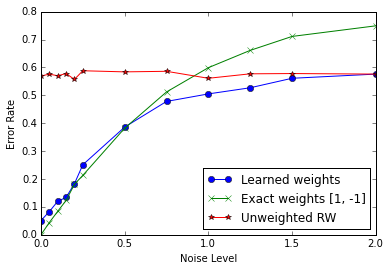
\includegraphics[width=\linewidth]{noise_plot}
\captionof{figure}{Error rate of destination set predicted by Supervised Random Walks and benchmarks. The noise variance ranges from $0$ (indicating no noise) to $2.0$.}
\label{fig:syn_noise}
\end{Figure}

Synthetic graphs with different noise levels are tested for prediction accuracy. In the graph without noise, we expect the learned parameter $\hat{\beta}$ to be very close to $\left[ 1, -1\right]$. As the noise level increases, the prediction accuracy may gradually decrease.

Accuracy is measured by error rate, which is calculated by the portion of true future destination set $D_{s}$ recovered by the predicted future destination set $\hat{D}_{s}$. To evaluate relative performance, we compare the error rates of Supervised Random Walks to using the true parameter $\left[ 1, -1\right]$ and unweighted random walk.

Fig. \ref{fig:syn_noise} demonstrates the performance of Supervised Random Walks compared to the benchmarks as noise variance increases from from $0$ (indicating no noise) to $2.0$. For each noise level, 10 independent graphs were generated and the average error rate for the 10 graphs is shown in the figure.

For synthetic graphs with no noise, Supervised Random Walks achieves near-zero error rate, as expected. As the noise level increases, Supervised Random Walk starts to outperform exact weights. This is because the learning process adapts to rising noise level, and is able to learn parameters that result in less error. Since unweighted random walk does not take node or edge features into account, its performance is stable across noise levels. The performance of Supervised Random Walks gradually approaches that of unweighted random walk as the noise level increases. This is expected, as node and edge features become poor predictors when the noise level is high, and graph characteristics come to dominate prediction performance.

Unlike the results reported in \cite{backstrom}, the error rate of Supervised Random Walks is slightly higher than the exact weights for low noise levels in our synthetic data. This is likely because we used a slightly looser convergence condition, making the recovered parameter $\beta$ less exact. However, such low noise is unlikely in real data, and so we believe this to be a reasonable trade-off for better computational feasibility.

\section{Repository Recommendation}

We will describe the Personalized PageRank-based method used to obtain repository recommendations for individual users using the repository graph computed by Supervised Random Walks and information about which repositories they have interacted with or contributed to.

\section{Evaluation}

We will describe our evaluation results. We will first compare the repository graph at the end of 12/31/2014 as computed by Supervised Random Walks against the true repository graph and graphs obtained by baseline methods (e.g. nearest neighbor). We will then compare the repository recommendations returned by Personalized PageRank for specific users (e.g. ones who have contributed to many repositories) against actual repositories contributed to. We will consider our method successful if the recommendations are an accurate predictor for the true contributions.

\section{Conclusion}

We will summarize our findings.

\begin{thebibliography}{9}
\bibitem{kleinberg} D. Liben-Nowell, J. Kleinberg. The Link Prediction Problem for Social Networks. In \textit{Proceedings of the Twelfth International Conference on Information and Knowledge Management}, 2004.
\bibitem{backstrom} L. Backstrom, J. Leskovec. Supervised Random Walks: Predicting and Recommending Links in Social Networks. In \textit{Proceedings of the Fourth ACM International Conference on Web Search and Data Mining}, 2011.
\bibitem{page}  L. Page, S. Brin, R. Motwani, T. Winograd. The
PageRank Citation Ranking: Bringing Order to the Web.
Technical report, Stanford InfoLab, 1999.
\bibitem{gha} \verb|https://www.githubarchive.org/|
\end{thebibliography}

\end{multicols}

\end{document}
